\xiti
\begin{xiaotis}

\xiaoti{}%
\begin{xiaoxiaotis}%
    \xxt[\xxtsep]{求证:直径是圆中最长的弦;}

    \xxt{如图,将卡钳的两脚张开,使两脚尖的距离等于规定的尺寸。
        当工件恰好通过两脚尖的张口时,表示它的直径符合规定;
        当工件不能通过或留有空隙时,它的直径不符合规定。为什么?
    }

\end{xiaoxiaotis}

\xiaoti{$\yuan\,O$ 的半径 $r = 5$ 厘米,圆心 $O$ 到直线 $l$ 的距离 $d = OD = 3$ 厘米。
    在直线 $l$ 上有 $P$、$Q$、$R$ 三点,且有 $PD = 4$ 厘米; $QD > 4$ 厘米;
    $RD < 4$ 厘米。它们对于 $\yuan\,O$ 的位置各是怎样的?
}

\xiaoti{求证:菱形各边的中点在同一个圆上。}

\xiaoti{已知: $AB = 4$ 厘米。以 3 厘米为半径作圆,使它经过点 $A$ 和 $B$。}

\xiaoti{作一个圆,使它经过已知点 $A$ 和 $B$,并且圆心在已知直线 $l$ 上。}
\begin{xiaoxiaotis}

    \xxt{当直线 $l$ 和 $AB$ 斜交时,可作出几个?}

    \xxt{当直线 $l$ 和 $AB$ 垂直但不经过 $AB$ 的中点时,可作出几个?}

    \xxt{当直线 $l$ 是线段 $AB$ 的垂直平分线时,怎样呢?}
\end{xiaoxiaotis}


\xiaoti{$\yuan\,O$ 的半径为 5 厘米,弦 $AB \pingxing CD$, $AB = 6$ 厘米,
    $OD = 8$ 厘米。 求 $AB$ 和 $CD$ 的距离(有两解)。
}

\xiaoti{经过已知 $\yuan\,O$ 内的已知点 $A$ 作弦,使它以点 $A$ 为中点。}

\begin{figure}[htbp]
    \centering
    \begin{minipage}[b]{4cm}
        \centering
        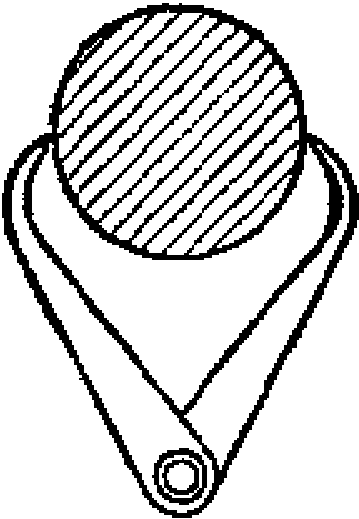
\includegraphics[width=2.5cm]{../pic/czjh2-ch7-xiti24-01.png}
        \caption*{(第 1 题)}
    \end{minipage}
    \qquad
    \begin{minipage}[b]{4cm}
        \centering
        \begin{tikzpicture}
    \tkzDefPoints{0/0/O}
    \tkzDefPoint(200:1.5){A}
    \tkzDefPoint(20:1.5){B}
    \tkzDefPoint(235:1.5){C}
    \tkzDefPoint(305:1.5){D}
    \tkzDefLine[altitude](C,A,D)  \tkzGetPoint{E}
    \tkzDefLine[altitude](C,B,D)  \tkzGetPoint{F}

    \tkzDrawCircle[thick](O,A)
    \tkzDrawSegments(A,B  A,E  B,F)
    \tkzDrawLine[add=0.1 and 0.1](E,F)
    \tkzDrawPoint(O)
    \tkzMarkRightAngle[size=.2](A,E,C)
    \tkzMarkRightAngle[size=.2](B,F,D)
    \tkzLabelPoints[above](O)
    \tkzLabelPoints[left](A)
    \tkzLabelPoints[right](B)
    \tkzLabelPoints[below](C)
    \tkzLabelPoints[below](D)
    \tkzLabelPoints[below left](E)
    \tkzLabelPoints[below right](F)
\end{tikzpicture}


        \caption*{(第 8 题)}
    \end{minipage}
    \qquad
    \begin{minipage}[b]{5cm}
        \centering
        \begin{tikzpicture}
    \pgfmathsetmacro{\factor}{0.025}
    \pgfmathsetmacro{\R}{130*\factor/2}
    \tkzDefPoints{0/0/O}
    \tkzDefPoint(180:\R){C}
    \tkzDefPoint(0:\R){D}
    \tkzDefPoint(90:\R){E}
    \tkzDefPointOnLine[pos=32/65](O,E)  \tkzGetPoint{F}
    \tkzDefLine[parallel=through F](C,D)  \tkzGetPoint{a}
    \tkzInterLC(F,a)(O,C)  \tkzGetPoints{B}{A}

    \tkzDrawCircle[thick](O,A)
    \tkzDrawArc[pattern={mylines[angle=65, distance={4pt}]}](O,B)(A)
    \tkzDrawSegments(A,B)
    \tkzDrawSegment[latex-latex](C,D)  \tkzLabelSegment[below](C,D){$\phi 130$}
    \tkzDrawPoint(O)

    \tkzLabelPoints[above](O)
    \tkzLabelPoints[left](A)
    \tkzLabelPoints[above, xshift=.5em](B)

    %
    \tkzDefPointOnLine[pos=1.4](F,B)  \tkzGetPoint{G}
    \tkzDefPointBy[translation=from F to G](E)  \tkzGetPoint{H}
    \tkzDefShiftPoint[G](0,-0.4){g}
    \tkzDefShiftPoint[H](0, 0.4){h}
    \tkzDrawLines[add=0 and 0.1](E,H  F,G)
    \tkzLabelSegment[rotate=90, yshift=.5em](G,H){$32$}  \tkzDrawSegments[-latex](g,G  h,H)
\end{tikzpicture}


        \caption*{(第 9 题)}
    \end{minipage}
    \qquad
\end{figure}

\xiaoti{如图,$AB$ 是 $\yuan\,O$ 的直径, $CD$ 是弦, $AE \perp CD$,垂足为 $E$;
    $BF \perp CD$, 垂足为 $F$。 求证: $EC = FD$。
}

\xiaoti{在直径为 130 mm 的圆铁片上切去一块高为 32 mm 的弓形铁片(如图)。
    求弓形的弦 $AB$ 的长。
}

\xiaoti{破残的轮片上,弓形的弦 $AB$ 长 480 mm, 高 $CD$ 为 70 mm(如图)。求原轮片的直径。}

\begin{figure}[htbp]
    \centering
    \begin{minipage}[b]{7cm}
        \centering
        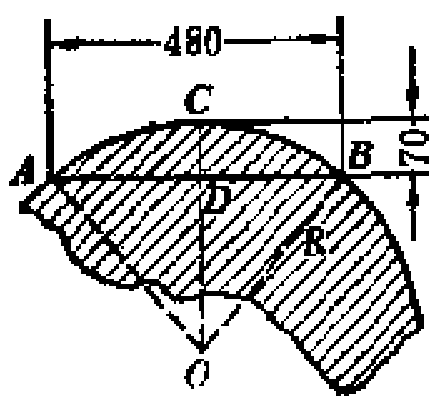
\includegraphics[width=4cm]{../pic/czjh2-ch7-xiti24-10.png}
        \caption*{(第 10 题)}
    \end{minipage}
    \qquad
    \begin{minipage}[b]{4cm}
        \centering
        \begin{tikzpicture}
    \tkzDefPoints{0/0/B, 2.5/0.5/C}
    \tkzDefTriangle[equilateral](B,C)  \tkzGetPoint{A}
    \tkzDefCircle[circum](A,B,C)  \tkzGetPoints{O}{R}
    \tkzDefTriangle[two angles=80 and 40](B,C)  \tkzGetPoint{P}

    \tkzDrawCircle[thick](O,R)
    \tkzDrawPolygon(A,P,B,C)
    \tkzDrawSegments(A,B  C,P)
    \tkzDrawPoint(O)
    \tkzLabelPoints[below](O)
    \tkzLabelPoints[above](A)
    \tkzLabelPoints[left](B)
    \tkzLabelPoints[right](C)
    \tkzLabelPoints[above](P)
\end{tikzpicture}


        \caption*{(第 14 题)}
    \end{minipage}
\end{figure}

\xiaoti{弦 $AB$ 和 $CD$ 相交于圆内的点 $P$,并且和经过点 $P$ 的直径成等角。求证: $AB = CD$。}

\xiaoti{}%
\begin{xiaoxiaotis}%
    \xxt[\xxtsep]{求证:经过 $\yuan\,O$ 内一点 $P$ 的所有弦中,与 $OP$ 垂直的弦最短;}

    \xxt{已知 $\yuan\,O$ 的半径为 6 厘米, $OP = 3.6$ 厘米。求经过点 $P$ 最短的弦长。}

\end{xiaoxiaotis}

\xiaoti{圆内接六边形 $ABCDEF$ 的各边相等,求各边所对的圆心角的度数。}

\xiaoti{已知:如图, $\angle APC = \angle CPB = 60^\circ$。
    求证: $\triangle ABC$ 是等边三角形。
}

\xiaoti{圆上一点 $P$ 到直径 $AB$ 的垂线的垂足为 $D$。求证: $\triangle BPD \xiangsi \triangle PAD$。}

\xiaoti{$\triangle ABC$ 中, $\angle BAC$ 的平分线与边 $BC$ 和外接圆分别相交于点 $D$ 和 $E$。
    求证: $\triangle ABD \xiangsi \triangle AEC$。
}

\xiaoti{求证:以等腰三角形的一腰为直径的圆,平分底边。}

\xiaoti{圆内接三角形 $ABC$ 中, $AB = AC$, 经过点 $A$ 的弦与 $BC$ 和 $\yuanhu{BC}$
    分别相交于点 $D$ 和 $E$。 求证: $\triangle ABD \xiangsi \triangle AEB$。
}

\xiaoti{使用曲尺检验工件的凹面,成半圆形时为合格。如图所示的三种情况中,
    哪种是合格的?哪种是不合格的?为什么?
}

\begin{figure}[htbp]
    \centering
    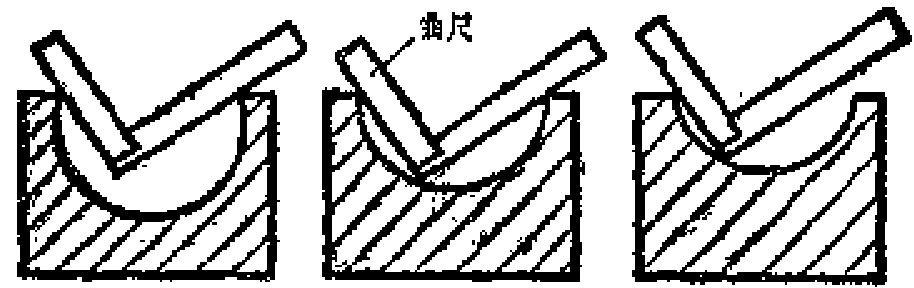
\includegraphics[width=8cm]{../pic/czjh2-ch7-xiti24-19.png}
    \caption*{(第 19 题)}
\end{figure}

\xiaoti{已知线段 $AB$ ,怎样作出几个点 $C_1$、$C_2$、…,使它们对 $AB$ 所张的角
    $\angle AC_1B$、$\angle AC_2B$、… 都是直角?
}

\xiaoti{圆内接四边形 $ABCD$ 中, $\angle A$、$\angle B$、$\angle C$ 的度数的比是 $2:3:6$。求四边形各内角的度数。}

\xiaoti{如图, $AD$ 是 $\triangle ABC$ 外角 $\angle EAC$ 的平分线,与三角形的外接圆交于点 $D$。求证: $DB = DC$。}

\begin{figure}[htbp]
    \centering
    \begin{minipage}[b]{5cm}
        \centering
        \begin{tikzpicture}
    \tkzDefPoints{0/0/O}
    \tkzDefPoint(120:1.5){A}
    \tkzDefPoint(225:1.5){B}
    \tkzDefPoint(315:1.5){C}
    \tkzDefPointOnLine[pos=1.4](B,A)  \tkzGetPoint{E}
    \tkzDefLine[bisector](C,A,E)  \tkzGetPoint{d}
    \tkzInterLC[common=A](A,d)(O,A)  \tkzGetFirstPoint{D}

    \tkzDrawCircle[thick](O,A)
    \tkzDrawPolygon(A,B,C)
    \tkzDrawSegments(A,C  A,D  A,E  B,D  C,D)
    \tkzLabelPoints[left, yshift=.5em](A)
    \tkzLabelPoints[left](B)
    \tkzLabelPoints[right](C)
    \tkzLabelPoints[above](D)
    \tkzLabelPoints[left](E)
\end{tikzpicture}


        \caption*{(第 22 题)}
    \end{minipage}
    \qquad
    \begin{minipage}[b]{6cm}
        \centering
        \begin{tikzpicture}
    \tkzDefPoints{0/0/B, 4/0/C, 1/2.5/A}
    \tkzDefLine[altitude](A,B,C)  \tkzGetPoint{E}
    \tkzDefLine[altitude](A,C,B)  \tkzGetPoint{F}

    \tkzDrawPolygon(A,B,C)
    \tkzDrawSegments(B,E  C,F  E,F)
    \tkzMarkRightAngle[size=.2](B,E,C)
    \tkzMarkRightAngle[size=.2](B,F,C)
    \tkzLabelPoints[above](A)
    \tkzLabelPoints[left](B,F)
    \tkzLabelPoints[right](C,E)
\end{tikzpicture}


        \caption*{(第 23 题)}
    \end{minipage}
\end{figure}

\xiaoti{已知: $BE$、$CF$ 是 $\triangle ABC$ 的两条高。 求证: $\angle AEF = \angle ABC$。}

\xiaoti{用反证法证明:}
\begin{xiaoxiaotis}

    \xxt{一个三角形的内角中,不能有两个钝角或直角;}

    \xxt{在同圆内,如果两条弦不等,那么它们的弦心距也不等;}

    \xxt{在同一平面内,一条直线与两条平行线中的一条相交,必定与另一条也相交。}

\end{xiaoxiaotis}



\end{xiaotis}

